\documentclass[12pt]{article}

\usepackage[utf8]{inputenc}%jsta
\usepackage[english]{babel}%test
\usepackage{float}

\usepackage{natbib}
\bibliographystyle{apalike}
\bibpunct[; ]{(}{)}{,}{a}{}{;}

\usepackage{Sweave}
\usepackage{pifont,mdframed}%test

\newenvironment{warning}
{\par\begin{mdframed}[linewidth=2pt,linecolor=red]
\begin{list}{}{\leftmargin=1cm
  \labelwidth=\leftmargin}\item[\Large\ding{43}]}
{\end{list}\end{mdframed}\par}

\usepackage{geometry}
\geometry{left=1.25in,right=1.25in,top=1.25in,bottom=1.25in}
\usepackage{rotating}
\usepackage{fancyhdr}
\usepackage[bookmarks,colorlinks,breaklinks,citecolor=red]{hyperref}

\usepackage{dirtree}%jsta
\usepackage{hyphenat}%jsta

%\usepackage{float}
\usepackage{graphicx,subfig}
% \usepackage{placeins}
\setlength\headheight{26pt}

\fancypagestyle{plain}{\fancyhf{}\fancyhead[R]{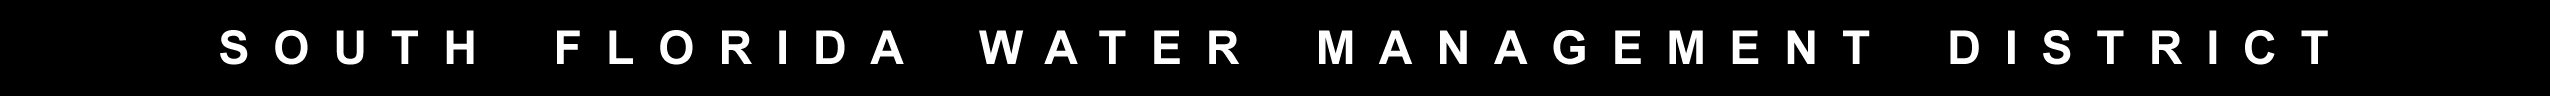
\includegraphics[width=6.0in,keepaspectratio=true]{sfwmd_bar8half_wordorexcel.png}}}

\author{Joseph Stachelek}
\title{Dataflow Output Standard Operating Procedure (SOP)}

%\VignetteIndexEntry{Dataflow Output Standard Operating Procedure(SOP)}

\begin{document}
\Sconcordance{concordance:DataflowR.tex:DataflowR.Rnw:%
1 62 1 1 2 4 0 1 2 94 1 1 2 4 0 1 2 5 1 1 2 4 0 1 2 5 1 1 2 4 0 1 2 8 1 %
1 2 4 0 1 2 4 1 1 2 4 0 1 2 14 1 1 2 4 0 1 2 4 1 1 2 4 0 1 2 4 1 1 2 4 %
0 1 2 14 1 1 2 4 0 1 2 15 1 1 2 4 0 1 2 6 1 1 2 4 0 1 2 7 1}

\maketitle
\tableofcontents
 
\vspace{15pt}
%\newpage
\section{Introduction}

This SOP details a workflow and introduces an \texttt{R} package to clean, load, interpolate, and plot streaming Dataflow output and associated discrete grab samples. The steps neccessary to perform a number of more involved data analyses are also included.

\section{Programs and Applications used in this SOP}

\begin{itemize}
  \item A spreadsheet program (MS Excel or similar)
  \item R (must have the \texttt{DataflowR} package and its dependencies installed) 
  \item RStudio (optional; for more easily accessing documentation)
  \item GRASS (optional; alternatively use QGIS, ArcGIS, Surfer, etc, for more easily adjusting final symbology)
\end{itemize}
 
\section{Installing the \texttt{DataflowR} package}

The \texttt{R} package \texttt{DataflowR} is distributed via a \texttt{.tar.gz} (analagous to \texttt{.zip}) package archive file. This package contains the source code for package functions as well as the archived datasets for the SFWMD Florida Bay Dataflow Monitoring Program. In RStudio, it can be installed by navigating to \texttt{Tools} -> \texttt{Install Packages...} -> \texttt{Install from:} -> \texttt{Package Archive File}. Computers running the Windows operating system can only install binary \texttt{.zip} package archive files unless they have additional compiler software installed. The \texttt{DataflowR} binary package can be installed by running the following command from the \texttt{R} console:

\begin{Schunk}
\begin{Sinput}
> install.packages(path.to.zip,type="win.binary",repos=NULL,dependencies = TRUE)
\end{Sinput}
\end{Schunk}

where \texttt{path.to.zip} is replaced by the file path of the \texttt{.zip} file. In most cases, \texttt{DataflowR} will be installed in the default user library in a folder named for your version of R. On Windows this is probably:\vspace{5pt}\\

\texttt{C:/Users/}\verb|<your_username>|\texttt{/Documents/R/win-library/}\verb|<your_R_version>|\texttt{/DataflowR}.\\

The directory should have the following file structure:

\dirtree{%
.1 /.
.2 doc.
.2 extdata.
.2 help.
.2 html.
.2 Meta.
.2 R.
}

\subsection{Data}

All data is stored under \texttt{extdata} in the following subdirectories:\\

\dirtree{%
.1 /.
.2 extdata.
.3 DF\_BaseFile.
.3 DF\_FullDataSets.
.3 DF\_Subsets.
.3 DF\_Surfaces.
.3 DF\_Validation.
}
\vspace{15pt}
\begin{warning}
\textcolor{red}{IMPORTANT!!} before continuing, copy the contents of \texttt{extdata} to a local folder such as: \verb|C:\Documents\Data\Dataflow|.\\ This will become your "working directory". Package functions will read and write to this directory without directly modifying archived datasets.\\ Next, update the first line of the file \texttt{localpath} to point to the location of this new folder.
For example, the structure of \verb|C:\Documents\Data\Dataflow| would look like:

\dirtree{%
.1 /.
.2 Dataflow.
.3 DF\_BaseFile.
.3 DF\_FullDataSets.
.3 DF\_Subsets.
.3 DF\_Surfaces.
.3 DF\_Validation.
}

\end{warning}

Dataflow surveys in the archived data respository include the following:

\begin{center}
\begin{tabular}{l*{10} {c} r}
\hline
Year & 15 & 14 & 13 & 12 & 11 & 10 & 09 & 08 & 07 & 06\\ \hline
J &  &  &  &  &  &  &  & x & x & \\
F & x & x &  &  & x & x &  &  &  & \\
M &  &  &  & x &  &  &  &  &  & \\
A &  & x &  &  &  & x & x & x &  & \\
M & x &  & x &  & x &  &  &  &  & x \\
J &  &  &  & x & x &  & x &  &  & \\
J & x & x &  &  &  & x &  &  & x & x \\
A &  &  & x & x &  &  &  & x &  & \\
S & x &  &  & x & x &  &  &  & x & x \\
O &  & x &  &  &  &  & x &  &  & \\
N &  &  & x &  &  &  &  &  &  & \\
D & x &  &  & x &  &  &  & x &  & \\
\hline
\end{tabular}
\end{center}

\subsection{GIS Software}
Some portions of \nameref{sec:plottingsurf} (Section 4.5) requires dedicated GIS software such as QGIS, ArcGIS, or GRASS GIS. In the interest of creating a fully reproducible and streamlined workflow for plotting Dataflow output some functions (\texttt{grassmap}) requires GRASS GIS (GRASS). GRASS can be installed by navigating to \href{http://grass.osgeo.org}{http://grass.osgeo.org}.

\vspace{15pt}
\begin{warning}
\texttt{DataflowR} assumes that the user is on a Linux machine and that GRASS is installed under \texttt{/usr/lib/grass70}. For more details see \citet{rgrass7}.
\end{warning}

\section{Handling streaming data}
\subsection{Cleaning incoming Dataflow and C6 files}

Incoming streaming data should be placed in \verb|DF_FullDataSets|\texttt{/Raw/InstrumentOutput} in a folder named for the survey date in yyyymm format (e.g. Feb-2015 is 201502). Likewise, Dataflow (\texttt{".txt"} or \texttt{".TXT"}) and C6 (\texttt{".csv"} or \texttt{".CSV"})  files should start with the survey date in yyyymmdd format. For example, the raw data files for February 2015 would be placed under:


\dirtree{%
.1 /.
.2 Dataflow.
.3 DF\_FullDataSets.
.4 Raw.
.5 InstrumentOutput.
.6 201502.
.7 20150211\_DF021115.txt.
.7 ....
.7 20150211\_C6\_11FEB.csv.
.7 ....
}
\begin{warning}
When working in a non-Windows environment, \texttt{.csv} files created under Windows may need to be opened and resaved as \texttt{text}\verb|\csv| in order to avoid illegal "nul" characters.
\end{warning}

\vspace{15pt}
Cleaning is accomplished via the \nohyphens{\texttt{streamclean}} function. The example below shows how to specify inputs to clean the data for the February 2015 survey. For this example we set the \texttt{tofile} parameter to \texttt{FALSE} but setting it to \texttt{TRUE} will save the cleaned output to \verb|DF_FullDataSets| as a \texttt{.csv} file. The \texttt{streamclean} function will gather all the Dataflow records, merge them with the C6 data, remove leading and trailing records of all zeros, format GPS coordinates, check that conductivity to salinity calculations are correct (recalculate if neccesary), and classify records based on fathom and CERP basin designations. Variable names and column ordering are formatted consistently and a machine readable (POSIX) date-time stamp is created.   

\begin{Schunk}
\begin{Sinput}
> dt<-streamclean(yearmon=201502,mmin=7,c6pres=TRUE,tofile=FALSE,sep=",")
\end{Sinput}
\end{Schunk}

Some older Dataflow surveys have undergone a "hand-cleaning" and are missing the raw inputs neccessary to run \texttt{streamclean}. In these instances, the \texttt{streamparse} function can be used to align the formatting of these files to resemble the output of \texttt{streamclean}. Specifically, the function creates a POSIX compliant date field, and reproduces the column names and ordering of a \texttt{streamclean} output. 

\begin{Schunk}
\begin{Sinput}
> dt<-streamparse(yearmon=201007,tofile=FALSE)
\end{Sinput}
\end{Schunk}


\subsection{QA cleaned streaming data}

The \texttt{streamclean} function does not perform detailed QA of individual parameter values or detect systematic bias. Systematic bias might occur because of sensor drift or failure. In these cases there may be data but it is "junk data". The \texttt{streamqa} function creates a series of diagnostic plots of the data. The user enters an interactive QA "session" to detect systematic biases and eliminate unrealsitic data spikes. The first set of dialogs steps through each variable and gives the user the opportunity to define a valid data range (flagging values outside this range). Define a range higher (or lower) than all values to flag all records for that particular variable. The second set of dialogs compares parameters that are shared between the Dataflow and C6 instrumentation. The user is given the opportunity to flag the C6 or the Dataflow version of a shared parameter. 

Cleaned data files are not modified directly. Instead, \texttt{streamqa} creates a matrix of the same size as the original data file and populates this matrix with flags. \texttt{streamqa} writes the "qafile" output to the \verb|DF_FullDataSets/QA| directory and names it as the date appended by "qa". Subsequent analyses can filter the full dataset based on these QA flags.

\begin{Schunk}
\begin{Sinput}
> streamqa(yearmon=201502)
\end{Sinput}
\end{Schunk}

\texttt{streamqa} can be run more than once. On the first run, a new "qafile" will be produced. Subsequent runs will pull the data (filtered by the previous qa) and edit the existing qafile.

\subsection{Loading previously cleaned streaming data}

The \texttt{streamget} function will retrieve previously cleaned data. The function looks for full data sets in the \verb|DF_FullDataSets| folder that match the specified \texttt{yearmon} survey date. The optional parameter \texttt{qa} is set to TRUE by default in order for \texttt{streamget} to filter the dataset by corresponding \texttt{streamqa} output. An example for the February 2015 survey is shown below.

\begin{Schunk}
\begin{Sinput}
> dt<-streamget(yearmon=201502,qa=TRUE)
\end{Sinput}
\end{Schunk}

\subsection{Interpolating cleaned data files}

The \texttt{streaminterp} function will interpolate a dataset that has been loaded into memory from the \texttt{streamclean} or \texttt{streamget} functions. Interpolations are performed using functions in the \texttt{ipdw} \texttt{R} package \citep{ipdw}. Variables to be interpolated must be specified as inputs to the \texttt{paramlist} paramter. If you have loaded your dataset to memory under the name \texttt{dt}, use \texttt{names(dt)} to see the available parameters. Enter one or more parameters as arguments to a character list. For example, to interpolate salinity only (as below) use \texttt{c("sal")}. Additional parameters can be appended. For example, to interpolate salinity and temperature use \texttt{c("sal","temp")}. Interpolation should take about 20 minutes plus about 2 minutes for each entry in \texttt{paramlist}. Raster surface output will be written to a subfolder of \verb|DF_Surfaces| named for the year and month of the survey in question.\\

\texttt{streaminterp} will first attempt to split the full data set into training and validation datasets. If these already exist in the \verb|DF_Subsets| and \verb|DF_Validation| folders, a warning will be printed and the pre-existing datsets will be used. Next, \texttt{streaminterp} will attempt to create a dedicated folder under \verb|DF_Surfaces| to hold all the interpolated surfaces for the given survey. If this folder already exists, \texttt{streaminterp} will print a warning but the function should proceed as normal (the warning can be disregarded).\\

More details regarding the interpolation procedure can be found in \cite{stachelek2015application}.

\begin{Schunk}
\begin{Sinput}
> streaminterp(dt,paramlist=c("sal"),yearmon)
\end{Sinput}
\end{Schunk}

\subsection{\label{sec:plottingsurf}Plotting interpolated surfaces}

\subsubsection{Quick plot with R graphics}

A quick visual inspection of interpolated outputs can be accomplished using the \nohyphens{\texttt{surfplot}} function. The \texttt{rnge} parameter takes either a single survey date or a list of two survey dates to specify a date range for plotting. More detailed publication quality maps should be produced using a dedicated GIS program such as ArcGIS,QGIS, or GRASS GIS.

\begin{Schunk}
\begin{Sinput}
> surfplot(rnge=c(201502),params=c("sal"))
\end{Sinput}
\end{Schunk}


% \begin{figure}[h!]
% \begin{center}
% 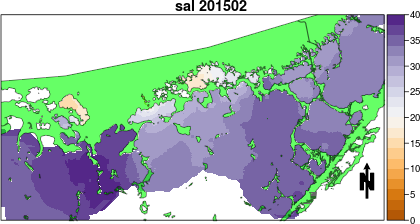
\includegraphics{figure0}
% \end{center}
% \label{fig:zero}
% \end{figure}
% %\FloatBarrier

\subsubsection{Detailed plotting with GRASS GIS}

The \texttt{grassmap} function creates detailed publication quality maps using GRASS GIS. Maps are output to the \verb|QGIS_plotting| folder. The following command creates a Bay-wide salinity map for May 2015.

\begin{Schunk}
\begin{Sinput}
> grassmap(rnge=201505,params=c("sal"))
\end{Sinput}
\end{Schunk}

\subsubsection{Producing timeseries for specific basins}

The \texttt{basin} parameter of the \texttt{grassmap} function allows the user to limit (zoom-in) to a specific FATHOM basin. A listing of FATHOM basins can be found by inspecting \verb|DF_Basefile/fathom_basins_proj.shp| or by referencing \citet{cosby2005fathom}. The following command will create a series of zoomed-in salinity maps of Manatee Bay for each survey date between June 2006 and May 2015.   

\begin{Schunk}
\begin{Sinput}
> grassmap(rnge=c(200605,201505),params=c("sal"),basin = "Manatee Bay")
\end{Sinput}
\end{Schunk}


\section{Handling discrete grab sample data}
\subsection{Cleaning grab sample records}
Incoming grab sample \texttt{.csv} data files should be placed in the \verb|DF_GrabSamples/Raw| folder and their file names should have the survey date in yyyymm format preappended. These files can be cleaned using the \texttt{grabclean} function. The \texttt{grabclean} function formats column names, removes columns/rows of missing data, and calculates minute averages of the streaming data that correspond to the grab sample date/times. Output is saved to the \verb|DF_GrabSamples| folder when \texttt{tofile} is set to \texttt{TRUE}. Suspect data records should be identified manually in the \texttt{flags} column. This becomes important in Section 6.2 because suspect data records can create problems converting between extracted and fluoresced chlorophyll.

\begin{Schunk}
\begin{Sinput}
> grabclean(yearmon=201410,tofile=FALSE)
\end{Sinput}
\end{Schunk}

\subsection{Loading previously cleaned grab data}

The \texttt{rnge} paramter takes either a single survey date or a list of two survey dates to specify a date range for retrieving cleaned grab data.

\begin{Schunk}
\begin{Sinput}
> grabs<-grabget(rnge=c(201402,201410))
\end{Sinput}
\end{Schunk}

\subsection{Plotting grab sample data}

Several plot types are defined in the \texttt{grabplot} function including "permit-style" vertical bar plots ("permitbarplot"), and.

\begin{Schunk}
\begin{Sinput}
> grabplot(rnge=201410,params=c("chla"),plottype="permitbarplot")
\end{Sinput}
\end{Schunk}
%\vspace{15pt}

 \begin{figure}[h!]
 \begin{center}
 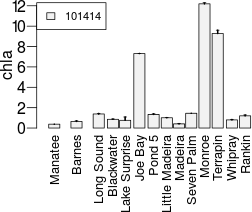
\includegraphics[width=3.5in,keepaspectratio=true]{figure1}
 \end{center}
 \label{fig:one}
 \end{figure}
%\clearpage
%\FloatBarrier

\section{Data Analysis}
\subsection{Calculating a difference-from-average surface}
The \texttt{avmap} function takes a survey date as input and searches the \verb|DF_Surfaces| folder for interpolated surfaces of the same parameter within a specified number of months for each year. The number of months on either side of the input month is set using the \texttt{tolerance} parameter. The found surfaces often have different extents. The \texttt{percentcov} parameter controls the percent of all identified surveys required before a pixel is included in difference-from-average computations. Output surfaces are written to the current working directory unless the \texttt{tofile} parameter is set to \texttt{FALSE}.

\begin{Schunk}
\begin{Sinput}
> avmap(yearmon=201502,params="sal",tofile=TRUE,percentcov=0.6,tolerance=1)
\end{Sinput}
\end{Schunk}

\begin{figure}[H]
\begin{center}
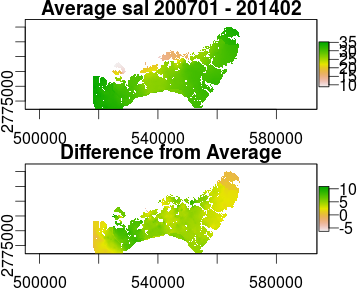
\includegraphics{figure2}
\end{center}
\label{fig:two}
\end{figure}
%\FloatBarrier

\subsection{Fit grab sample and streaming averages}
\subsubsection{Calculate coefficients}

In order to generate maps of chlorophyll concentration, streaming fluorescence values (chlorophyll, algal pigments, cdom) must be statistically "fit" (regressed) against lab-derived extracted chlorophyll values. The \texttt{chlcoef} function searches the \verb|DF_GrabSamples| folder for a cleaned grab dataset that matches the specified \texttt{yearmon} parameter value. First, the function generates a correlation matrix and identifies streaming variables that have at least a 0.4 correlation with extracted chlorophyll. The resulting variables are entered into a linear regression. If the R\textsuperscript{2} value of the regression is less than 0.7, the variables are entered into a second degree polynomial regression. The regression (either the linear or the second degree polynomial) is subjected to a backward stepwise AIC model selection \citep{mass}. The output of this step is usually a regression with a reduced number of parameters. The final regression is checked for multicolinearity by calculating variance inflation factors (vif) and excluding parameters until all vif values are less than 10 \citep{hh2002}. The previous steps, which include summaries of all intermediate model fits, are printed to the R console for inspection. 

The final set of variable coefficients, the R\textsuperscript{2} value, the p-value, and the formula for the final fitted equation are printed (appended) to the \texttt{extractChlcoef.csv} file in the \verb|DF_GrabSamples| folder.

\begin{Schunk}
\begin{Sinput}
> chlcoef(yearmon=201502,remove.flags=TRUE)
\end{Sinput}
\end{Schunk}

\subsubsection{Generate extracted chlorophyll surfaces}

The coefficients calculated as a result of the \texttt{chlcoef} function can be used to create an interpolated map of chlorophyll concentration. The \texttt{chlmap} function takes these coefficients and the associated fulldataset and calculates an extracted chlorophyll value for each measurement point ("extchl"). These values are interpolated using the \texttt{streaminterp} function. The output surface is stored in the \verb|DF_Surfaces| folder under the appropriate survey date folder.  

\begin{Schunk}
\begin{Sinput}
> chlmap(yearmon=201502)
\end{Sinput}
\end{Schunk}


\medskip
 \addcontentsline{toc}{section}{References}
 %\setlength{\bibsep}{0pt}
\bibliography{bib}
 
\end{document}
